\documentclass[11pt]{article}
\usepackage[a4paper,margin=1in]{geometry}
\usepackage{amsmath,amssymb,amsthm,mathtools}
\usepackage{booktabs}
\usepackage{graphicx}
\usepackage{hyperref}
\usepackage[nameinlink,capitalise]{cleveref}
\usepackage[numbers,sort&compress]{natbib}

\newtheorem{theorem}{Theorem}[section]
\newtheorem{proposition}[theorem]{Proposition}
\newtheorem{corollary}[theorem]{Corollary}
\theoremstyle{remark}
\newtheorem{remark}[theorem]{Remark}
\newcommand{\norm}[1]{\left\lVert#1\right\rVert}
\newcommand{\cR}{\mathcal R}

\title{Ky Fan Tail Majorization and a Weaker Endpoint Corridor to Stage A\\
\large Captured Energy, Rank Staircases, and Seven-Scale Stress Evidence}
\author{Liang Wang}
\date{July 2026}

\begin{document}
\maketitle

\begin{abstract}
RH-83 proved that termwise singular-value majorization is sufficient for an
optimal endpoint factorization, but dyadic singular staircases make that
condition stronger than the downstream problem requires.  This paper isolates
the weaker invariant that RH-78 actually uses: the Hilbert--Schmidt energy
left outside a low-rank postblock space.

For a Hilbert--Schmidt operator $B$ with Gramian $G=B^*B$, Ky Fan's principle
gives
\[
 \tau_r(B)^2
 =\operatorname{tr}G-\sum_{j=1}^r\lambda_j(G)
 \le \norm{B(I-P)}_2^2
\]
for every rank-$r$ orthogonal projector $P$.  Thus a validated captured-energy
lower bound certifies the optimal tail without resolving each singular value.

If the physical postblock state satisfies the tail-majorization condition
\[
 \tau_{J_\sigma+\ell}(B_\sigma)
 \le \alpha_\sigma
 \tau_{J_\sigma+\ell}(\cR_\sigma)+\varepsilon_\sigma,
\]
then RH-82 immediately yields an exponential excess-rank tail.  Polylogarithmic
$\alpha_\sigma$, remainder, and observability bounds close the RH-78
effective-rank corridor.  This condition neither identifies coordinates nor
controls the leading singular values, and is strictly weaker than the RH-83
factorization gate.

The numerical audit keeps the five 192-bit interval-certified postblock tails
and adds two out-of-sample levels: $\sigma=0.005$ at dimension $1024$ and
$\sigma=0.0025$ at dimension $2048$.  The clock rank grows only from four to
eight.  At every level the physical clock-plus-two tail is below $1.4\%$ of
the linear endpoint-model tail.  The largest interval-certified relative
tail is $2.34\times10^{-7}$; the two extended binary64 stress tails are below
$1.56\times10^{-15}$.

The result narrows the all-level problem to a captured-energy theorem for a
clock-dimensional postcritical packet space.  The two new levels are
diagnostic, not a proof of uniformity.  Stage A1, unconditional Stage A4,
Hilbert--Polya, and the Riemann Hypothesis remain open.
\end{abstract}

\noindent\textbf{Keywords:} Ky Fan principle; singular-value tail; effective
rank; captured energy; postblock state; small noise.

\medskip
\noindent\textbf{MSC 2020:} 47B10; 47A75; 15A18; 65G20.

\section{Why termwise majorization is more than needed}

The RH-83 optimal factorization theorem compares every leading physical
singular value with the corresponding endpoint singular value
\citep{WangSingularFactor2026}.  This is natural for an operator
factorization, but individual ratios can jump when a new singular staircase
enters between neighboring dyadic scales.  RH-78 does not use those ratios.
It uses only the residual left after a low-rank approximation
\citep{WangEffectiveRank2026}.

RH-82 already supplies the mediator estimate
\begin{equation}
 \tau_{J_\sigma+\ell}(\cR_\sigma)
 \le C_Rq^\ell,
 \qquad J_\sigma=\frac{\log(1/\sigma)}{2\log\lambda}+O(1),
 \label{eq:endpoint-tail}
\end{equation}
with $0<q<1$ \citep{WangHalfLog2026}.  The question is how little information
about $B_\sigma$ is required to inherit this tail.

\section{Ky Fan certification of a postblock tail}

Let $B:\mathcal H_1\to\mathcal H_2$ be Hilbert--Schmidt and let
$G=B^*B$.  Define
\[
 \tau_r(B)=\inf_{\operatorname{rank}L\le r}\norm{B-L}_2.
\]

\begin{theorem}[Ky Fan captured-energy upper]
\label{thm:kyfan}
For every integer $r\ge0$,
\begin{equation}
 \tau_r(B)^2
 =\operatorname{tr}G-\sum_{j=1}^r\lambda_j(G).
 \label{eq:optimal-tail}
\end{equation}
If $P$ is any rank-$r$ orthogonal projection on $\mathcal H_1$, then
\begin{equation}
 \boxed{
 \tau_r(B)^2\le\norm{B(I-P)}_2^2
 =\operatorname{tr}G-\operatorname{tr}(PG).}
 \label{eq:candidate-tail}
\end{equation}
\end{theorem}

\begin{proof}
The first identity is the Eckart--Young formula.  Ky Fan's maximum principle
states
\[
 \operatorname{tr}(PG)
 \le\sum_{j=1}^r\lambda_j(G).
\]
Subtract from $\operatorname{tr}G$ to obtain
\eqref{eq:candidate-tail} \citep{Bhatia1997}.
\end{proof}

The theorem is suited to interval work: one may fix a floating candidate
subspace and evaluate the residual directly in rigorous arithmetic.  No
interval eigendecomposition of the tiny tail eigenvalues is required.

\section{Tail-majorization transfer}

\begin{theorem}[Weak endpoint tail corridor]
\label{thm:transfer}
Suppose that for a rank schedule $r_\sigma=J_\sigma+\ell_\sigma$,
\begin{equation}
 \tau_{r_\sigma}(B_\sigma)
 \le\alpha_\sigma\tau_{r_\sigma}(\cR_\sigma)
 +\varepsilon_\sigma.
 \label{eq:tail-majorization}
\end{equation}
Then
\begin{equation}
 \boxed{
 \tau_{r_\sigma}(B_\sigma)
 \le\alpha_\sigma C_Rq^{\ell_\sigma}
 +\varepsilon_\sigma.}
 \label{eq:transferred-tail}
\end{equation}
If $\alpha_\sigma$, $\varepsilon_\sigma$, and the square root of the future
observability norm are polylogarithmic, then a logarithmic or
polylogarithmic $r_\sigma$ satisfies the RH-78 effective-rank residual gate.
\end{theorem}

\begin{proof}
Insert \eqref{eq:endpoint-tail} into
\eqref{eq:tail-majorization}.  Multiplication by the future observability
factor transfers the Hilbert--Schmidt residual to the directional Hardy
future exactly as in RH-77.
\end{proof}

This is strictly weaker than an RH-83 factorization.  A factorization implies
\eqref{eq:tail-majorization} by the ideal property, but a tail inequality says
nothing about the leading singular vectors or even their individual sizes.

\section{Seven-scale audit}

The first five levels retain the 192-bit Arb residuals from RH-82.  The audit
then builds two new frozen matrices at constant spatial resolution per noise
width:
\[
 (\sigma,n,M)=(0.005,1024,49),
 \qquad(0.0025,2048,64).
\]
These horizons continue the proposed log-square schedule.  They are not an
analytic horizon theorem.

For each channel, the endpoint model uses the linear powered-row Gram matrix
and the physical rank is
\begin{equation}
 r_\sigma=\lceil H_\sigma\rceil+2.
 \label{eq:rank}
\end{equation}

\begin{table}[ht]
\centering
\small
\begin{tabular}{rrrrr}
\toprule
$\sigma$ & fine dimension & rank & max physical/endpoint tail & evidence\\
\midrule
0.16 & 32 & 4 & $1.393\times10^{-2}$ & Arb\\
0.08 & 64 & 5 & $3.814\times10^{-6}$ & Arb\\
0.04 & 128 & 6 & $9.969\times10^{-7}$ & Arb\\
0.02 & 256 & 6 & $5.143\times10^{-6}$ & Arb\\
0.01 & 512 & 7 & $9.257\times10^{-7}$ & Arb\\
0.005 & 1024 & 8 & $4.687\times10^{-12}$ & binary64 stress\\
0.0025 & 2048 & 8 & $1.050\times10^{-12}$ & binary64 stress\\
\bottomrule
\end{tabular}
\caption{Maximum over both directional channels.  Only the first five
physical tails are interval certified.}
\label{tab:audit}
\end{table}

The worst ratio occurs at the coarsest scale.  At smaller noise the physical
tail is much smaller than the already small endpoint tail.  The ambient
dimension grows by a factor $64$, while the tested rank only doubles.

\begin{figure}[ht]
\centering
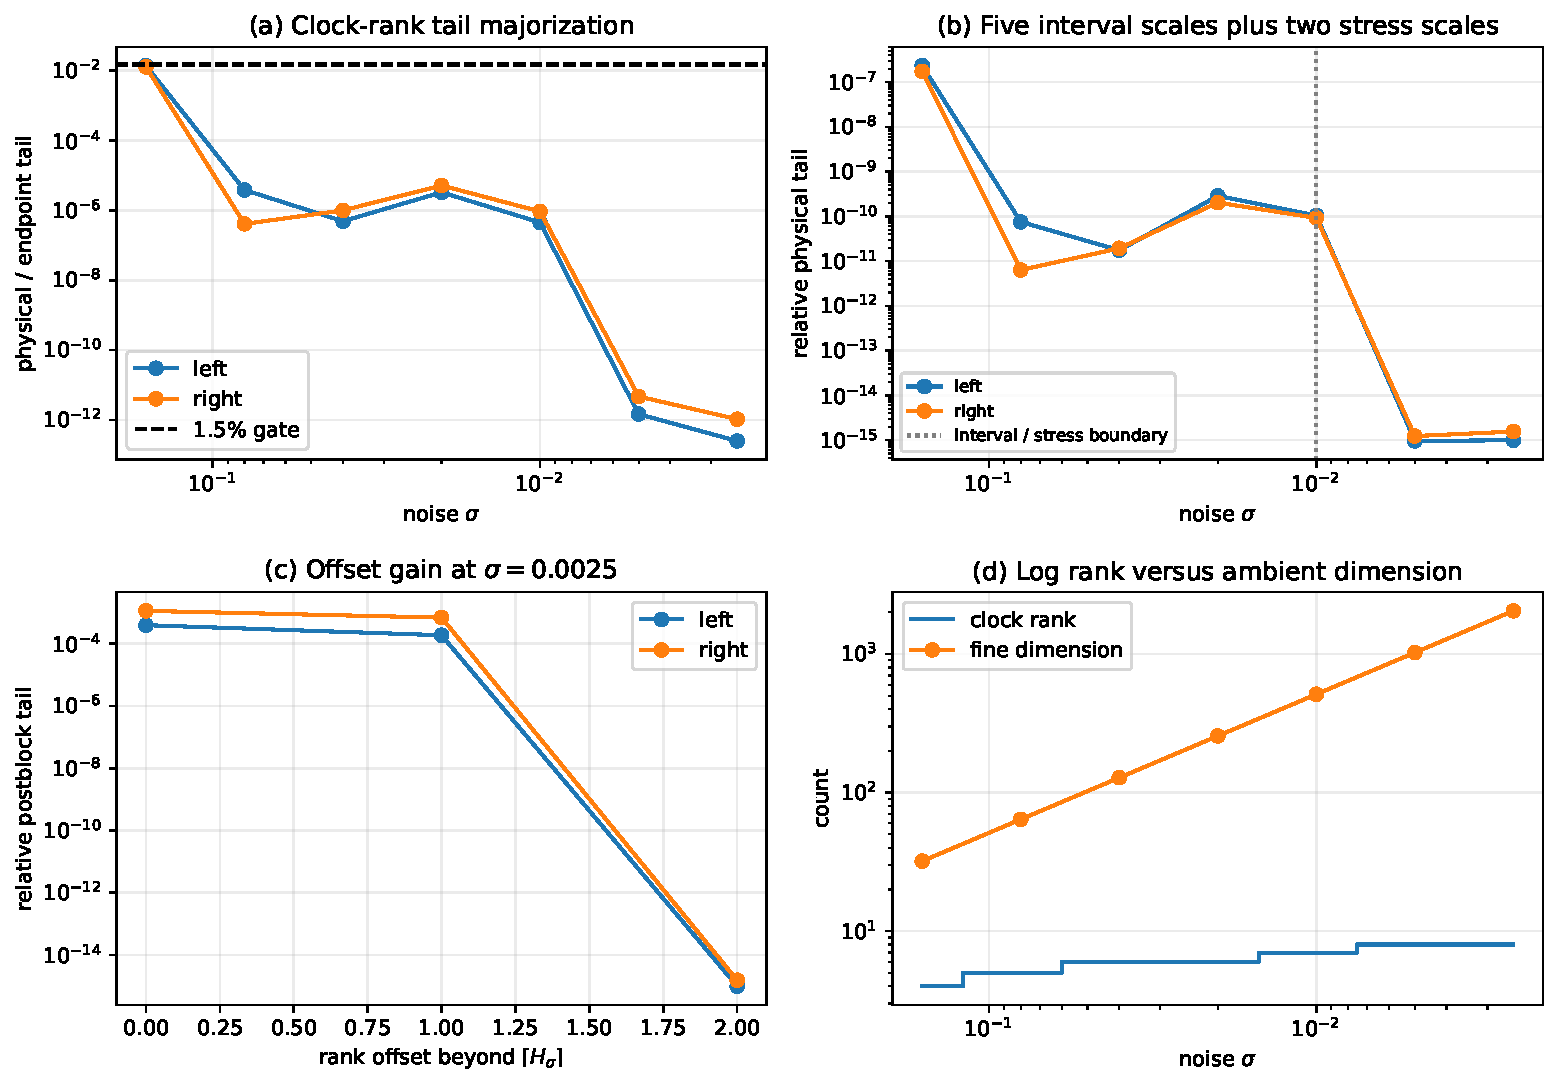
\includegraphics[width=\textwidth]{figures/ky_fan_tail_majorization.pdf}
\caption{Tail-majorization ratios, interval and stress residuals, excess-rank
gain at the finest level, and logarithmic rank versus ambient dimension.}
\label{fig:tail}
\end{figure}

\section{Next theorem and boundary}

The all-level target can now be stated without singular-value matching:
construct a rank-$O(\log(1/\sigma))$ postcritical packet projector
$P_\sigma$ and prove
\begin{equation}
 \operatorname{tr}(P_\sigma B_\sigma^*B_\sigma)
 \ge\norm{B_\sigma}_2^2
 -\operatorname{polylog}(1/\sigma)^2.
 \label{eq:captured-energy-target}
\end{equation}
Combined with \cref{thm:kyfan}, this is enough.  The packet vectors may be
rotated by the dynamics; they need not equal sampled endpoint rows.

This paper proves the Ky Fan and tail-transfer theorems and validates the
five inherited interval scales plus two floating stress levels.  It does not
prove \eqref{eq:captured-energy-target} uniformly, close Stage A1 or
unconditional Stage A4, construct an A5 relative determinant, produce a
self-adjoint Hilbert--Polya operator, derive a $T\log T$ or prime-power law,
identify zeta zeros, or prove the Riemann Hypothesis.

\bibliographystyle{plainnat}
\bibliography{references}

\end{document}

